\documentclass{standalone}
\usepackage{tikz}
\usetikzlibrary{positioning,fit,arrows}
\begin{document}
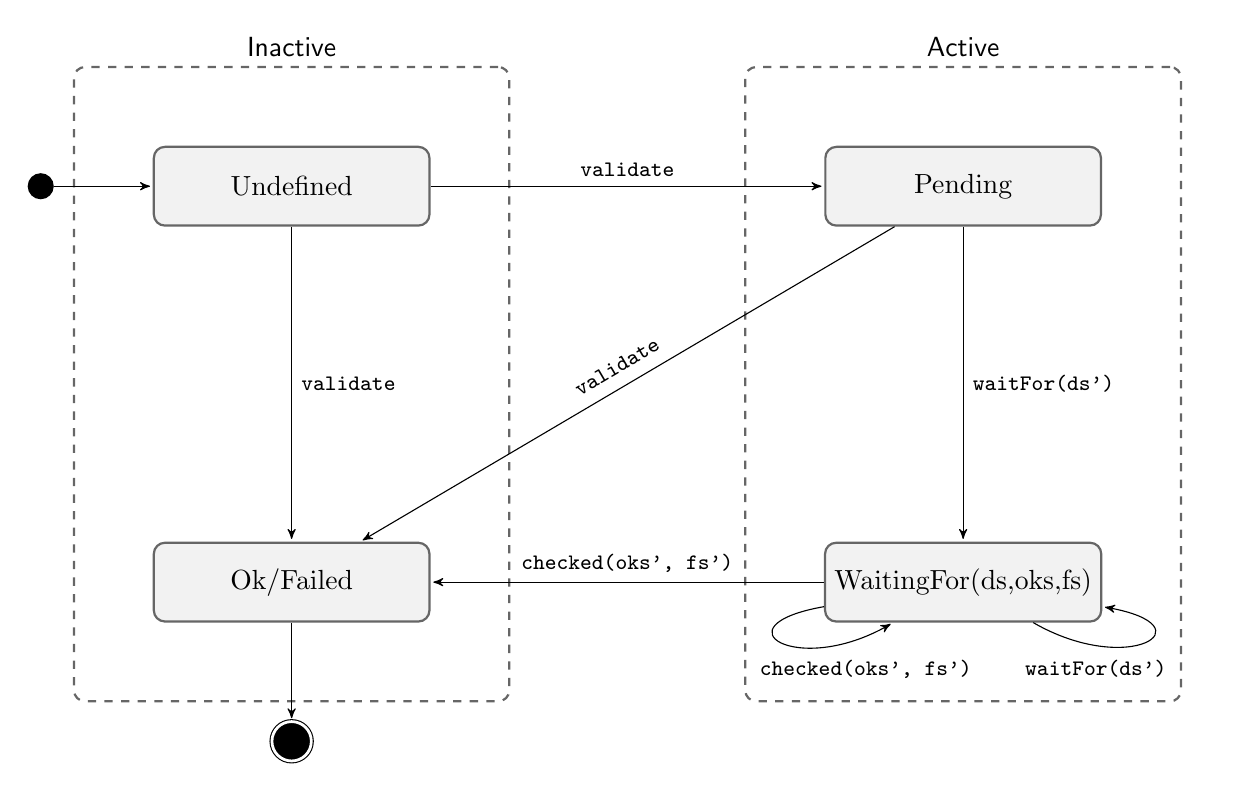
\begin{tikzpicture}[
        state/.style={
                rectangle,
                rounded corners,
                draw=black!60,
                fill=black!5,
                thick,
                minimum width=35mm,
                minimum height=10mm
            },
        initial/.style={
                circle,
                fill=black,
                minimum size=3mm
            },
        accepting/.style={
                circle,
                draw,
                double=black!0,
                double distance=1pt,
                fill=black,
                draw=black,
                minimum size=5mm
            },
        array/.style={
                rectangle,
                rounded corners,
                draw=black!60,
                dashed,
                thick
            },
        predicate/.style = {font=\footnotesize\ttfamily},
        >= stealth',
        shorten >= 1pt
    ]
    \node[state] (unknown)                        {Undefined};
    \node[state] (pending) [right=5cm of unknown] {Pending};
    \node[state] (ok)      [below=4cm of unknown] {Ok/Failed};
    \node[state] (waiting) [below=4cm of pending] {WaitingFor(ds,oks,fs)};
    \node[initial] (initial) [left=1.25cm of unknown]  {};
    \node[accepting] (accepting) [below=1.25cm of ok]  {};

    \node[array,fit={(unknown)(ok)},draw,inner sep=1cm,label={[font=\sffamily]Inactive}] (inactive) {};
    \node[array,fit={(pending)(waiting)},draw,inner sep=1cm,label={[font=\sffamily]Active}] (active) {};

    \path[->] (initial) edge node {} (unknown);
    \path[->] (ok) edge node {} (accepting);
    \path[->] (unknown) edge node[predicate, above] {validate} (pending);
    \path[->] (unknown) edge node[predicate, right] {validate} (ok);
    \path[->] (pending) edge node[predicate, sloped, above=0.05cm] {validate} (ok);
    \path[->] (pending) edge node[predicate,right] {waitFor(ds')} (waiting);
    \path[->] (waiting) edge node[predicate, above] {checked(oks', fs')} (ok);
    \path[->] (waiting) edge[out=190,in=210,looseness=4] node [predicate, below right=0.1cm and -0.4cm] {checked(oks', fs')} (waiting);
    \path[->] (waiting) edge[out=330,in=350,looseness=4] node [predicate, below left=0.1cm and -0.4cm] {waitFor(ds')} (waiting);
\end{tikzpicture}
\end{document}